% Author: Izaak Neutelings (October 2020)
% https://mathworld.wolfram.com/PhasePortrait.html
\documentclass[border=3pt,tikz]{standalone}
\usepackage{amsmath} % for \dfrac
\usepackage{physics,siunitx}
\usepackage{tikz,pgfplots}
\usepackage[outline]{contour} % glow around text
\contourlength{1.0pt}
\usetikzlibrary{angles,quotes} % for pic (angle labels)
\usetikzlibrary{arrows.meta}
\usetikzlibrary{decorations.markings}
%\usetikzlibrary{bending} % for arrow head angle
\tikzset{>=latex} % for LaTeX arrow head
\usepackage{xcolor}

\colorlet{xcol}{blue!60!black}
\colorlet{myred}{red!80!black}
\colorlet{myblue}{blue!80!black}
\colorlet{mygreen}{green!40!black}
\colorlet{myorange}{orange!90!black}
\colorlet{mypurple}{red!50!blue!90!black!80}
\colorlet{mydarkred}{myred!80!black}
\colorlet{mydarkblue}{myblue!80!black}
\tikzstyle{xline}=[xcol,thick]
\tikzstyle{width}=[{Latex[length=5,width=3]}-{Latex[length=5,width=3]},thick]
\tikzset{
  traj/.style 2 args={xline,postaction={decorate},decoration={markings,
    mark=at position #1 with {\arrow{<}},
    mark=at position #2 with {\arrow{<}}}
  }
}
\def\tick#1#2{\draw[thick] (#1)++(#2:0.12) --++ (#2-180:0.24)}
\def\N{100} % number of samples


\begin{document}
% COS - overdamped
% https://en.wikipedia.org/wiki/Harmonic_oscillator#Universal_oscillator_equation
% https://brilliant.org/wiki/damped-harmonic-oscillators/
% https://beltoforion.de/en/harmonic_oscillator/
% http://hyperphysics.phy-astr.gsu.edu/hbase/oscda.html#c1
% http://hyperphysics.phy-astr.gsu.edu/hbase/oscda2.html#c1
% https://ocw.mit.edu/courses/mathematics/18-03sc-differential-equations-fall-2011/unit-ii-second-order-constant-coefficient-linear-equations/damped-harmonic-oscillators/MIT18_03SCF11_s13_2text.pdf
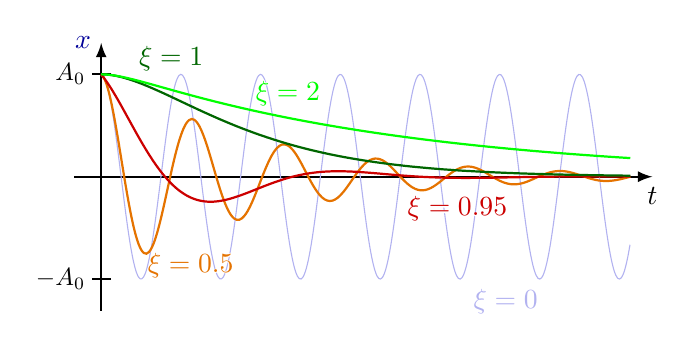
\begin{tikzpicture}
  \def\xmax{7.0} % max x axis
  \def\ymax{1.7} % max y axis
  \def\A{1.3}
  \def\om{(6.5/(0.94*\xmax))} % natural omega_0
  \def\Za{0.50} % zeta underdamped 1
  \def\Zb{0.95} % zeta underdamped 2
  \def\Zc{1.00} % zeta critically damped
  \def\Zd{2.00} % zeta overdamped
  \def\Ga{(\Za*\om)} % gamma underdamped 1
  \def\Gb{(\Zb*\om)} % gamma underdamped 2
  \def\Gc{\om}       % gamma critically damped
  \def\Gd{(\Zd*\om)} % gamma overdamped
  \def\Wa{(\om*sqrt(1-\Za*\Za)}  % omega underdamped 1
  \def\Wb{(\om*sqrt(1-\Zb*\Zb)}  % omega underdamped 2
  \def\Wd{(\om*sqrt(\Zd*\Zd-1))} % omega overdamped
  
  % AXIS
  \draw[->,thick] (0,-\ymax) -- (0,\ymax) node[left,xcol] {$x$};
  \draw[->,thick] (-0.2*\ymax,0) -- (\xmax,0) node[below] {$t$};
  \tick{0,\A}{0} node[left=-1,scale=0.9] {$A_0$};
  \tick{0,-\A}{0} node[left=-1,scale=0.9] {$-A_0$};
  
  % PLOT
  \draw[xline,myblue!30,thin,samples=200+\N,smooth,variable=\t,domain=0:0.96*\xmax]
    plot(\t,{\A*cos(360*\om*\t)});
  \draw[xline,myorange,samples=100+\N,smooth,variable=\t,domain=0:0.96*\xmax]
    plot(\t,{\A*exp(-\Ga*\t)*cos(360*\Wa*\t)});
  \draw[xline,myred,samples=\N,smooth,variable=\t,domain=0:0.96*\xmax]
    plot(\t,{\A*exp(-\Gb*\t)*cos(360*\Wb*\t)});
  \draw[xline,mygreen,samples=\N,smooth,variable=\t,domain=0:0.96*\xmax]
    plot(\t,{\A*(1+\Gc*\t)*exp(-\Gc*\t)});
  \draw[xline,green,samples=\N,smooth,variable=\t,domain=0:0.96*\xmax]
    plot(\t,{\A/2*( (1+\Gd/\Wd)*exp((\Wd-\Gd)*\t) + (1-\Gd/\Wd)*exp(-(\Wd+\Gd)*\t))});
  %\node[above=4] at (0.15*\xmax,{\A*exp(-0.15*\xmax/\T)}) {$e^{-\frac{b}{2m}t}$};
  
  % NODES
  \node[below,myblue!30] at ({5.20*\om},-1.00*\A) {$\xi=0$};
  \node[below,myorange]   at ({1.15*\om},-0.65*\A) {\contour{white}{$\xi=0.5$}};
  \node[below,myred]     at ({4.58*\om},-0.10*\A) {\contour{white}{$\xi=0.95$}};
  \node[above,mygreen]   at ({0.90*\om}, 0.94*\A) {$\xi=1$};
  \node[above,green]      at ({2.40*\om}, 0.60*\A) {\contour{white}{$\xi=2$}};
  
\end{tikzpicture}
\end{document}